\part{Implementación}\label{part:implementacion}

\section{Hardware}

\section{Programa del microcontrolador} \label{sec:sw-implementacion}

\subsubsection{Archivo principal} \label{sec:archivo_principal}

\lstinputlisting[label=pseudo:userInit, linerange=1-10, firstnumber=1] {codigo/pseudocodigo/microcontrolador.pseudo}

El Archivo principal del programa que corre sobre el microcontrolador es el archivo main.cpp.
Dentro tiene un método denominado \code{user\_init()} que actúa como punto de entrada de la aplicación y no contiene parámetros.
En su definición se inicializa cada clase mencionada en la sección previa, ejecutando el método init( ) de cada una de ellas.
Dicho método es el encargado de asignar los valores iniciales a las variables internas de cada módulo de software, de forma de poder usar sus servicios públicos, posteriormente.
Éstas clases son las que se observan en la figura \ref{fig:flujo_de_datos}: WiFiManager, LedSign, Server y Settings.

Adicionalmente se establece tasa de bits por segundo a 115200 por medio de una función propia del SDK utilizado para el desarrollo.
Por último para utilizar los pines del micro, se inicializan los GPIO del microcontrolador, a través de la función gpio\_init( ) que también es propia del SDK.
En el fragmento \ref{pseudo:userInit} se muestra un pseudocódigo del método user\_init\( \).

Por último, se observa que para la clase Settings, se ejecuta el método loadSettings( ).
El mismo se encarga de cargar desde la memoria no volátil del microcontrolador, la última información almacenada respecto del texto a mostrar en el cartel, sus parámetros de configuración, y sus valores de red. \newline

\subsubsection{Settings}

La clase Settings es la encargada de mantener en memoria RAM, la información principal respecto del cartel.
Entre ellas, contiene el texto a mostrar, su velocidad de parpadeo y desplazamiento y la información de la red a la que actualmente se encuentra conectado el sistema.
Además posee funcionalidades para almacenar dichos datos en memoria no volátil a fin de persistirlos ante un reinicio.
En la figura \ref{uml:settings}, se observa un diagrama UML con los principales métodos de la clase en cuestión, y a continuación se describe cada uno de ellos.

\begin{figure}[!ht]
	\centering
	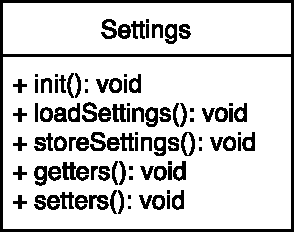
\includegraphics[scale=0.8]{imagenes/uml/settings.pdf}
	\caption{UML de la clase Settings.}
	\label{uml:settings}
\end{figure}

\lstinputlisting[linerange=12-12, firstnumber=12] {codigo/pseudocodigo/microcontrolador.pseudo}

El método \code{init()} de settings se encarga de inicializar el puntero de la estructura de la flash de donde lee y almacena los datos.
Adicionalmente, la clase provee funcionalidad para establecer las configuraciones por defecto del sistema, presionando el botón de RST durante 5 segundos.
Para lograr eso, dentro del método \code{init()} también se inicializa el pin que se va a utilizar como reset (pin GPIO2) y se establece el callback para cuando dicho evento ocurra.
Se recomienda revisar la sección \ref{sec:sdk} donde se explica el mecanismo de callbacks que utiliza el microcontrolador.

\lstinputlisting[linerange=14-14, firstnumber=14] {codigo/pseudocodigo/microcontrolador.pseudo}

El método \code{loadSettings()} se encarga de cargar en memoria RAM la información necesaria del cartel utilizando el puntero previamente incializado en \code{init()}.
Adicionalmente se le envía, dicha información, a la clase LedSign quien es la encargada de mostrar el contenido anteriormente almacenado en la memoria.

En caso de que la información leída estuviese corrupta, la clase contiene un método privado para cargar los datos por defecto del sistema.
El método no posee parámetros.

\lstinputlisting[linerange=16-16, firstnumber=16] {codigo/pseudocodigo/microcontrolador.pseudo}

El método \code{storeSettings()} de la clase Settings provee funcionalidad para almacenar en la memoria no volátil la información actual del sistema.
Para la persistencia de los datos, se utiliza la librería propietaria del SDK denominada spi\_flash.h.
Este método no contiene parámetros.


\subsubsection{WiFiManager}

La clase WiFiManager es la encargada de administrar todas las configuraciones WiFi que necesita el microcontrolador para conectarse a una red.
Posee un sólo método público enunciado en el apartado \ref{sec:archivo_principal}, denominado init( ).

\lstinputlisting[linerange=18-18, firstnumber=18] {codigo/pseudocodigo/microcontrolador.pseudo}

El método no contiene parámetros y su principal tarea consiste en leer los datos de la clase Settings relacionados a la información de la red.
Dichos valores corresponden al SSID, contraseña de WiFi, ip, y máscara de subred y son utilizados para permitir al sistema conectarse a la red WiFi correspondiente.
La librería propia del SDK osapi.h permite realizar estas acciones.



\subsubsection{Server}

Una vez conectado a la red WiFi, la clase Server es la encargada de colocar al microcontrolador en modo servidor, de forma de poder atender las peticiones que realiza el usuario.
Provee funcionalidades para inicializar el servidor, desconectar la sesión, enviar mensajes hacia el cliente, y notificar cuando se recibe un paquete.
En el UML de la figura \ref{uml:server} se observan los métodos públicos de la clase que abstrae las funcionalidades mencionadas anteriormente.

\begin{figure}[!ht]
	\centering
	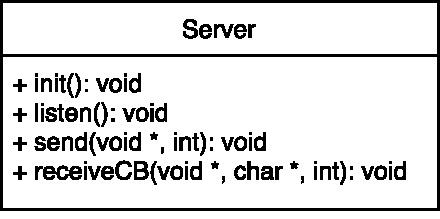
\includegraphics[scale=0.8]{imagenes/uml/server.pdf}
	\caption{UML de la clase Server.}
	\label{uml:server}
\end{figure}

Cabe destacar que en la figura \ref{uml:server} aparece una función privada relacionada a la recepción de mensajes denominada \code{receiveCallback()}.
Como bien su nombre lo indica, esto es un callback que se setea dentro del método \code{listen()} y se ejecuta cuando algún paquete llega al servidor (para más información, revisar la sección \ref{sec:sdk} donde se explica el método de callbacks).
A pesar de que sea un método privado, se decide mostrar en el UML debido a su reelevancia en esta solución.
Más adelanete, en esta sección, se explica su implementación.

\lstinputlisting[linerange=20-20, firstnumber=20] {codigo/pseudocodigo/microcontrolador.pseudo}

El método \code{init()} de la clase Server se ejecuta en el archivo principal y su función esencial consiste en inicializar las variables internas de la estructura de modo de permitir, posteriormente, colocar al microcontrolador en modo servidor.
Cabe aclarar que esta función debe ejecutarse después de haberse autenticado a una red WiFi; por ese motivo, primero se ejecta el \code{init()} de la clase WiFiManager.
Por otra parte, éste método no coloca al programa en modo servidor, es decir, no permite que distintos clientes se conecten todavía; para ello debe ejecutarse el método \code{listen()} que se describe a continuación.

\lstinputlisting[linerange=22-22, firstnumber=22] {codigo/pseudocodigo/microcontrolador.pseudo}

En primer lugar, el método \code{listen()} configura el certificado y la clave de seguridad del protocolo SSL que se utiliza en el intercambio de mensajes entre el servidor y el cliente de forma de que los mismos permanezcan cifrados hasta llegar a destino.
Adicionalmente, activa el mecanismo de Keep Alive propio de TCP, limita el número de conexiones simultáneas a uno y registrar los callbacks necesarios para su correcto funcionamiento (entre ellos el correspondiente a la recepción de paquetes).
El método no contiene parámetros.

\lstinputlisting[linerange=24-24, firstnumber=24] {codigo/pseudocodigo/microcontrolador.pseudo}

El método \code{send()} provee funcionalidad para enviar mediante TCP, hacia el cliente, un arreglo de bytes de manera cifrada.
Para su utilización, es necesario haber ejecutado el método \code{listen()} previamente y haber establecido una conexión con un cliente.

Recibe como parámetro un puntero que contiene la dirección del mensaje a enviar y el tamaño de dicho paquete.

\lstinputlisting[label=pseudo:receiveCallback, linerange=26-32, firstnumber=26] {codigo/pseudocodigo/microcontrolador.pseudo}

Como ya se mencionó anteriormente, el método \code{receiveCallback()} es una función privada que se ejecuta sólo cuando se reciben datos desde el cliente (size).
Contiene un buffer interno donde almacena los bytes que obtiene.
Los parámetros que recibe corresponden con la conexión vía TCP que envía los datos (conn), un puntero a la cadena de bytes recibido (data) y por último el tamaño de dicho arreglo.

Dicha estructura posee una capacidad limitada y, en este caso, su tamaño máximo se especifica en el protocolo de software (ver sección \ref{sec:protocolo}).
Cabe aclarar que la tarea de este método es acumular bytes hasta llenar el buffer. La clase Server no tiene las herramientas necesarias para interpretar la información que recibe.
Por ese motivo cuando la estructura se llena, se notifica a la clase MessageHandler quien es la que implementa el protocolo de comunicación diseñado para este proyecto y es quien es capaz de interpretar la secuencia de bytes recibida.



\subsubsection{MessageHandler}

La clase MessageHandler implementa el protocolo de comunicación entre el servidor y el cliente, y es capaz de interpretar el arreglo de bytes que recibe desde la clase Server.
Esta clase contiene un sólo método denominado \code{handle()} que atiende el mensaje que le envía el usuario y genera una respuesta para el cliente.
En el fragmento \ref{pseudo:messageHandlerHandle} se muestra un pseudocódigo del método a fin de brindar mayor claridad en la comprensión de la función.

\lstinputlisting[label=pseudo:messageHandlerHandle,linerange=36-93, firstnumber=36] {codigo/pseudocodigo/microcontrolador.pseudo}



\subsubsection{LedSign}

La última clase de la arquitectura del programa del microcontrolador es LedSign.
La misma se encarga de recibir los datos que envía MessageHandler por parámetro, procesarlos y armar un buffer de salida con la información necesaria para encender las luces de la matriz.
Cabe recordar que el programa del microcontrolador solo se comunica con el primer MAX7219 como lo indica la figura \ref{fig:flujo_de_datos}.
En la figura \ref{uml:ledSign} se muestra un UML con los métodos públicos que componen la clase.

\begin{figure}[!ht]
	\centering
	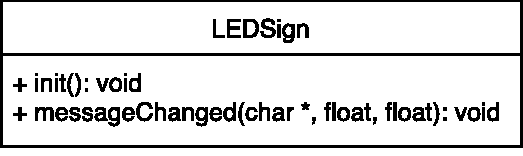
\includegraphics[scale=0.8]{imagenes/uml/LEDSign.pdf}
	\caption{UML de la clase LEDSign.}
	\label{uml:ledSign}
\end{figure}

\lstinputlisting[linerange=95-109, firstnumber=95] {codigo/pseudocodigo/microcontrolador.pseudo}

En primer lugar, el método \code{init()} se encarga de configurar los pines LATCH, CLK y DATA que se utilizan para la comunicación entre el microcontrolador y el MAX7219.
Para mayor información respecto de los pines, se sugiere visitar la sección \ref{sec:hw} %TODO AMG - poner la sección donde se explica los pines esos.

Adicionalmente se configura como salida los pines que se utilizan para los jumpers, se les habilita su pull up interno y se lee su valor a la salida.
De esta forma, se indica cuántos módulos de 8x8 LEDs componen el cartel.

Por otra parte, el método se encarga de configurar todos los registros necesarios de cada MAX7219 para iniciar su funcionamiento.
Entre las acciones que realiza, el programa se encarga de sacarlo del modo test, configurar la intensidad de los LEDs, indicarle que se van a usar las ocho columnas que posee el chip, limpiarle la pantalla apagando todos los LEDs y encenderlo.
Dichas configuraciones se realizan través del método \code{sendCommand()}.
La función toma dos parámetros, en el primero se especifica el registro a configurar y en el segundo el valor que se desea establecer.
Para más información respecto de la configuración de los registros consultar el datasheet del MAX7219 haciendo click en el siguiente \href{https://datasheets.maximintegrated.com/en/ds/MAX7219-MAX7221.pdf}{link}.

Finalmente se limpia el cartel, apagando todas las luces de cada módulo.

\lstinputlisting[linerange=111-111, firstnumber=111] {codigo/pseudocodigo/microcontrolador.pseudo}

El método \code{messageChanged()} se invoca cuando el mensaje o algún parámetro de configuración (tiempo de parpadeo o velocidad de desplazamiento) es modificado.

Recibe tres parámetros de configuración, el primero es el texto a mostrar.
Éste es un puntero a char donde se encuentra la información del contenido.
Es necesario que tenga un terminador nulo.
En caso de que no lo tenga, el comportamiento del método queda indefinido.

El segundo parámetro es brate, es un float que indica la velocidad de parpadeo que posee el texto.
Un valor negativo, repercute en comportamiento indefinido.
En caso de que no se requiera se debe colocar un 0.

El último parámetro es srate que también es un float que indica la velocidad a la que se desplaza el contenido.
La diferencia con el anterior radica en que este sí puede tomar valores negativos.
Un valor negativo indica que el contenido se desplaza a la izquierda, mientras que un positivo lo hace hacia la derecha.
En caso de que no se requiera el uso de esta funcionalidad, se debe colocar un 0. 

La función principal de este método es tomar los datos de configuración que se reciben por parámetro y armar un buffer de salida con la información de cada columna del cartel, respecto del estado de cada LED.
Para realizar el desplazamineto del contenido, la estrategia que se adopta es periódicamente, mover el índice del buffer y enviar nuevamente la información al MAX7219.
Para el tiempo se utiliza una estructura propia del SDK del microcontrolador denominado timer\_t.
La misma permite ejecutar un callback cuando se cumple un determinado lapso de tiempo.

Para realizar el parpadeo del mensaje, se adopta una estrategia similar.
Basándose en otro timer\_t se envía periódicamente un comando a cada MAX7219 que le indica que debe encenderse o apagarse, según corresponda.

\section{Aplicación de PC}
